\documentclass[11pt]{article}

\usepackage[margin=1in]{geometry}
\usepackage[T1]{fontenc}
\usepackage{lmodern}
\usepackage{amsmath,amssymb,amsthm,mathtools}
\usepackage{hyperref}
\usepackage{enumitem}
\usepackage{microtype}
\usepackage{graphicx}

\raggedbottom
\allowdisplaybreaks[2]

\setlength{\parindent}{1.5em}
\setlength{\parskip}{0pt}
\setlength{\abovedisplayskip}{7pt plus 2pt minus 3pt}
\setlength{\belowdisplayskip}{7pt plus 2pt minus 3pt}
\setlength{\abovedisplayshortskip}{4pt plus 2pt minus 2pt}
\setlength{\belowdisplayshortskip}{4pt plus 2pt minus 2pt}

\setlist{topsep=3pt,itemsep=2pt,parsep=0pt,partopsep=0pt}

\hypersetup{
colorlinks=true,
linkcolor=blue,
citecolor=blue,
urlcolor=blue
}

\newtheoremstyle{tightplain}
{6pt}{6pt}{\itshape}{}{\bfseries}{.}{.5em}{}
\newtheoremstyle{tightdef}
{6pt}{6pt}{}{}{\bfseries}{.}{.5em}{}

\theoremstyle{tightplain}
\newtheorem{theorem}{Theorem}[section]
\newtheorem{proposition}[theorem]{Proposition}
\newtheorem{lemma}[theorem]{Lemma}
\newtheorem{corollary}[theorem]{Corollary}

\theoremstyle{tightdef}
\newtheorem{assumption}[theorem]{Assumption}
\newtheorem{remark}[theorem]{Remark}
\newtheorem{definition}[theorem]{Definition}

\DeclareMathOperator{\tr}{tr}
\DeclareMathOperator{\diag}{diag}
\DeclareMathOperator{\rank}{rank}
\DeclareMathOperator{\op}{op}
\DeclareMathOperator{\KL}{KL}

\newcommand{\E}{\mathbb E}
\newcommand{\Prob}{\mathbb P}
\newcommand{\R}{\mathbb R}
\newcommand{\norm}[1]{\left\lVert #1 \right\rVert}
\newcommand{\abs}[1]{\left\lvert #1 \right\rvert}
\newcommand{\one}{\mathbf 1}
\newcommand{\F}{\mathrm F}
\newcommand{\dsub}{\mathfrak d_{\mathrm{sub}}}
\newcommand{\ssum}{\mathsf s}
\newcommand{\iid}{\stackrel{\mathrm{iid}}{\sim}}

\title{Overlap-Driven Subspace Drift in Rolling Covariance Windows}
\date{\today}

\begin{document}

\maketitle


\begin{abstract}
We analyze adjacent increments of top-$r$ spectral projectors computed from
rolling sample covariance matrices. Adjacent windows of length $W$ share
$W-1$ observations, so their covariance difference is driven only by the
entering and exiting boundary observations and has rank at most two. Under a
static Gaussian bulk-plus-spikes null, conditioning on the shared core yields:
conditional exchangeability of the two adjacent projectors; an exact one-pair
sign-randomization calibration for oriented projector contrasts; a null
fluctuation benchmark of order $r/W^2$; and, in the fixed-rank strongly spiked
regime, the leading expansion
\[
\E\norm{\widehat P_t-\widehat P_{t-1}}_F^2
=\frac{2}{\alpha_W^2}\frac{\dsub(\Sigma,r)}{W^2}
+o(W^{-2})
=
\frac{2\dsub(\Sigma,r)}{(W-1)^2}
+o(W^{-2}),
\]
where $\alpha_W=(W-1)/W$ and $\dsub$ is the spectral difficulty of
Definition~\ref{def:dsub}. Thus the common shorthand
$2\dsub(\Sigma,r)/W^2$ is asymptotically correct, while
$2\dsub(\Sigma,r)/(W-1)^2$ is the more accurate finite-$W$ leading
benchmark. Because the population subspace is fixed under the null, this
constant is a noise floor for detecting genuine subspace movement, not a
measure of drift itself. We also give a boundary-driven least-favorable family
showing that this $r/W^2$ scale is sharp for the corresponding rolling drift
target.
\end{abstract}

\section{Introduction}

\subsection{The adjacent subspace increment}

Let $\{r_s\}$ be a sequence of mean-zero random vectors in $\R^n$, let
$I_t=\{t-W+1,\ldots,t\}$ denote the rolling window of length $W$ ending at time
$t$, and define the rolling sample covariance
\[
\widehat\Sigma_t=\frac1W\sum_{s\in I_t}r_s r_s^\top.
\]
For a symmetric matrix $A$ with a positive top-$r$ eigengap, let $P(A)$ denote
its top-$r$ spectral projector, and write $\widehat P_t=P(\widehat\Sigma_t)$.
The object of this paper is the \emph{adjacent subspace increment}
\[
\widehat P_t-\widehat P_{t-1}.
\]
Our focus is neither the covariance estimate itself nor single-window principal
component analysis, but the increment of the estimated principal subspace
between two consecutive windows. The windows $I_{t-1}$ and $I_t$ overlap in
$W-1$ observations, so that
\begin{equation}\label{eq:rank2}
\widehat\Sigma_t-\widehat\Sigma_{t-1}
=\frac1W\bigl(r_t r_t^\top-r_{t-W}r_{t-W}^\top\bigr).
\end{equation}
Although each estimate $\widehat\Sigma_t$ is built from $W$ observations, their
difference has rank at most two and depends only on the entering observation
$r_t$ and the exiting observation $r_{t-W}$. The rank-two boundary identity
\eqref{eq:rank2} is the source of the faster decay rate that we establish for
the adjacent increment.

\subsection{Related work}

Principal subspaces and spectral projectors of covariance matrices are central
objects in multivariate statistics. Their behavior in high dimensions has been
studied extensively under the spiked covariance model of Johnstone
\cite{Johnstone2001}; see Paul \cite{Paul2007} and Benaych-Georges and
Nadakuditi \cite{BenaychNadakuditi2011} for the eigenstructure of low-rank
perturbations of large random matrices. Finite-sample and minimax theory for
principal subspace estimation includes Vu and Lei \cite{VuLei2013}, Cai, Ma and
Wu \cite{CaiMaWu2013}, and Cai and Zhang \cite{CaiZhang2018}. The underlying
perturbation theory for spectral projectors goes back to Davis and Kahan
\cite{DavisKahan1970}, Wedin \cite{Wedin1972}, and Kato \cite{Kato1995}; see
also Stewart and Sun \cite{StewartSun1990} and Bhatia \cite{Bhatia1997}. Sharp
operator-norm concentration for sample covariance operators in terms of
effective rank is due to Koltchinskii and Lounici \cite{KoltchinskiiLounici2017}.

Rolling-window covariance and subspace estimates are widely used to track
time-varying second-order structure and to localize changes in covariance
\cite{AueEtAl2009,WangYuRinaldo2021}. In such analyses the temporal overlap
between consecutive windows is typically not exploited. The present paper
isolates the effect of this overlap on the projector increment and shows that,
under a static null, it produces a drift scale smaller by one factor of $W$
than the single-window estimation error.

The scope is intentionally narrow. The exact exchangeability and one-pair
sign-calibration statements use an i.i.d.\ boundary pair independent of the
shared core; serial dependence or local nonstationarity can break the swap
argument unless the data are first blocked, resampled, or modeled so that an
exchangeable boundary experiment remains valid. Likewise, the constant-level
expansion is proved in a strongly spiked regime with fixed $r$ spikes of order
$n$, an $O(1)$ bulk, and a gap of order $n$, so the effective rank is $O(1)$
and the rates are dimension-free in this class. These assumptions are natural
for the clean null calculation, but they are substantive modeling restrictions
for rolling-window applications.

\subsection{Contributions}

We work under a static Gaussian bulk-plus-spikes null, made precise in
Section~\ref{sec:setup}. Under this null the population subspace does not move,
so the increment $\widehat P_t-\widehat P_{t-1}$ is pure estimation noise, and
its size is the natural benchmark against which true subspace drift must be
detected. Our contributions are the following.
\begin{enumerate}
\item \emph{Conditional exchangeability}
(Proposition~\ref{prop:exchangeability}). Conditional on the shared core of
$W-1$ common observations, the two adjacent projectors are independent and
identically distributed; in particular the increment is conditionally
mean-zero.
\item \emph{Exact one-pair randomization calibration}
(Theorem~\ref{thm:exactrandomization} and Corollary~\ref{cor:signtest}). Any
antisymmetric functional of a fixed adjacent projector pair --- in particular
any linear contrast of $\widehat P_t-\widehat P_{t-1}$ whose contrast is
measurable with respect to the shared core --- has a sign-symmetric conditional
law. This gives an exact one-pair randomization calibration for oriented
contrasts. It is intentionally a coarse single-pair calibration; using many
overlapping rolling times additionally requires blocking, a dependence argument,
or resampling calibration.
\item \emph{Adjacent-window null-increment benchmark}
(Theorem~\ref{thm:overlapbenchmark}). The expected squared Frobenius increment
is of order $r/W^2$, in contrast to the single-window projector error of order
$r/W$.
\item \emph{Constant-level expansion}
(Theorem~\ref{thm:adjacentconstantproved}). In the fixed-rank strongly spiked
Gaussian regime, the operative finite-$W$ leading approximation is
\[
\E\norm{\widehat P_t-\widehat P_{t-1}}_F^2
= \frac{2}{\alpha_W^2}\frac{\dsub(\Sigma,r)}{W^2}
+o(W^{-2})
=\frac{2\,\dsub(\Sigma,r)}{(W-1)^2}+o(W^{-2}).
\]
The limiting shorthand $2\mathfrak d_{\mathrm{sub}}/W^2$ is asymptotically
equivalent. This is a regime-specific Gaussian constant, not a universal
high-dimensional PCA constant.
\item \emph{Boundary-driven least-favorable sharpness}
(Proposition~\ref{prop:rollinglower} and Remark~\ref{rem:matchingupper}). A
boundary-driven hypercube gives a minimax lower bound of order $r/W^2$ for the
rolling drift target
$D_t^{\mathrm{roll}}=P(\bar\Sigma_t)-P(\bar\Sigma_{t-1})$. Over that same
local family the drift itself is at the null scale, so the zero estimator
matches the lower-bound rate. This section should therefore be read as a
sharpness statement at the null floor, not as a claim of nontrivial recovery
below that floor.
\end{enumerate}
Standard perturbation and concentration results used as inputs are collected in
Section~\ref{sec:aux}.

\subsection{Notation}

For a symmetric matrix $A$, $\lambda_1(A)\ge\cdots\ge\lambda_n(A)$ are its
ordered eigenvalues, $\norm{A}_{\op}$ its operator norm, $\norm{A}_F$ its
Frobenius norm, and $\langle A,B\rangle_F=\tr(A^\top B)$ the Frobenius inner
product. We write $a\lesssim b$ if $a\le Cb$ for a constant $C$ depending only
on the fixed spectral constants and the rank $r$, $a\asymp b$ if $a\lesssim b$
and $b\lesssim a$, and $a=\Theta(b)$ analogously. For a Hilbert-space-valued
random variable $X$ and a sub-$\sigma$-algebra $\mathcal G$,
\[
V_F(X\mid\mathcal G)
:=\E\bigl[\norm{X-\E[X\mid\mathcal G]}_F^2\bigm|\mathcal G\bigr]
\]
is the conditional Frobenius variance.

\section{Setup}\label{sec:setup}

Let $P(A)$ denote the top-$r$ spectral projector of a symmetric matrix $A$
whenever it is uniquely defined. On null sets with eigenvalue ties, fix any
measurable tie-breaking convention. The static-null results below use the
following i.i.d. Gaussian model.

\begin{assumption}[Static Gaussian null]\label{ass:gaussian}
On $I_t\cup I_{t-1}$, the vectors $r_s$ are independent and identically
distributed as $N(0,\Sigma)$.
\end{assumption}

\begin{assumption}[Bulk-plus-spikes spectrum]\label{ass:bulkspike}
The rank parameter $r$ is fixed. Eigenvalues are ordered as
\[
\lambda_1(\Sigma)\ge\lambda_2(\Sigma)\ge\cdots\ge\lambda_n(\Sigma).
\]
There exist constants $0<m<M<\infty$ and $0<c_\lambda\le C_\lambda<\infty$,
independent of $n$ and $W$, such that
\[
m\le \lambda_n(\Sigma)\le\cdots\le\lambda_{r+1}(\Sigma)\le M,
\qquad
c_\lambda n\le \lambda_r(\Sigma)\le\cdots\le\lambda_1(\Sigma)\le C_\lambda n.
\]
\end{assumption}

\begin{assumption}[Population eigengap]\label{ass:gap}
Let $\delta=\lambda_r(\Sigma)-\lambda_{r+1}(\Sigma)$. Assume
\[
\delta\ge c_\delta n.
\]
\end{assumption}

\begin{assumption}[Asymptotic convention]\label{ass:asymptotic}
The spike rank $r$ is fixed, $n$ may grow, and $W=W_n\to\infty$. Whenever
exponential sample-covariance concentration is invoked in a theorem statement,
we assume $W\ge C_{\log}\log n$ and $W\ge W_0$, with constants $C_{\log}$ and $W_0$ depending only on the fixed
spectral constants and on $r$. This global convention is stronger than
what the effective-rank concentration input alone requires; it is retained to
make all later high-probability and union-bound statements uniform.
\end{assumption}

The bulk-plus-spikes scaling of Assumption~\ref{ass:bulkspike} places the model
in the spiked regime studied by Johnstone \cite{Johnstone2001} and Paul
\cite{Paul2007}: $r$ spikes of order $n$ separated from an $O(1)$ bulk by a gap
of order $n$. This is the benign, well-separated regime; the consequences of
relaxing it are discussed in Remark~\ref{rem:scope}.

\section{Auxiliary standard inputs}\label{sec:aux}

We collect the standard perturbation and concentration results used in the
sequel. They are stated in the form convenient for our purposes and are
included to keep the paper self-contained.

\begin{lemma}[First-order projector expansion]\label{lem:projectorexpansion}
Let $A=A^\top$ have eigen-decomposition
\[
A=\sum_{k=1}^n \mu_k v_kv_k^\top,
\qquad
\mu_1\ge\cdots\ge\mu_n,
\]
and suppose the top-$r$ eigengap $\gamma=\mu_r-\mu_{r+1}$ is positive. Let
$P(A)$ be the top-$r$ spectral projector of $A$. Define the reduced-resolvent
derivative
\[
\mathcal L_A(E)
=\sum_{i\le r<j}
\frac{v_j v_j^\top E\, v_i v_i^\top+v_i v_i^\top E\, v_j v_j^\top}{\mu_i-\mu_j}.
\]
There exist constants $c_0\in(0,1/4]$ and $C_r<\infty$, depending at most on the
fixed rank $r$, such that if $\norm{E}_{\op}\le c_0\gamma$, then the top-$r$
projector $P(A+E)$ is uniquely defined and
\[
\norm{P(A+E)-P(A)-\mathcal L_A(E)}_F
\le
C_r\frac{\norm{E}_{\op}^2}{\gamma^2}.
\]
Consequently,
\[
\norm{P(A+E)-P(A)}_F
\le
C_r\frac{\norm{E}_{\op}}{\gamma}.
\]
\end{lemma}

\begin{proof}
Let $P=P(A)$ and write $\widetilde P=P(A+E)$. By Weyl's inequality
\cite[Ch.~III]{Bhatia1997}, if $\norm E_{\op}\le \gamma/4$ then the top-$r$
spectral cluster of $A+E$ remains separated from the lower cluster by at least
$\gamma/2$, so $\widetilde P$ is uniquely defined. We use the standard local
perturbation expansion for spectral projectors across an isolated gap
\cite{Kato1995,DavisKahan1970}: the map $H\mapsto P(A+H)$ is twice Fr\'echet
differentiable on the operator-norm ball $\norm H_{\op}\le\gamma/4$, its
derivative at zero is the reduced-resolvent operator $\mathcal L_A$, and
\[
\norm{D^2P(A+H)[B_1,B_2]}_{\op}
\le
C\frac{\norm{B_1}_{\op}\norm{B_2}_{\op}}{\gamma^2}
\]
for all $\norm H_{\op}\le\gamma/4$. This is the standard second-order bound for
spectral projectors across an isolated spectral gap; equivalently, it follows
from the Riesz-projector (contour-integral) representation
\cite[Ch.~II]{Kato1995} using any contour that strictly separates the top-$r$
cluster from its complement.

Taylor's formula therefore gives
\[
\norm{P(A+E)-P(A)-\mathcal L_A(E)}_{\op}
\le
C\frac{\norm E_{\op}^2}{\gamma^2}.
\]
The linear term has the displayed coordinate form by differentiating the
spectral projector in the eigenbasis of $A$. Finally, $P(A+E)-P(A)$ is the
difference of two rank-$r$ projectors and has rank at most $2r$, while
$\mathcal L_A(E)$ has only the two off-diagonal blocks between $P$ and
$P^\perp$ and rank at most $2r$. Hence the remainder has rank at most $4r$, so
\[
\norm{P(A+E)-P(A)-\mathcal L_A(E)}_F
\le
2\sqrt r\,\norm{P(A+E)-P(A)-\mathcal L_A(E)}_{\op}
\le
C_r\frac{\norm E_{\op}^2}{\gamma^2}.
\]
The final Lipschitz bound follows from
$\norm{\mathcal L_A(E)}_F\le C_r\norm E_{\op}/\gamma$ and the remainder bound,
after decreasing $c_0$ if necessary.
\end{proof}

\begin{lemma}[Gaussian operator-moment tools]\label{lem:covopmoments}
Let $S_N=N^{-1}\sum_{k=1}^N x_kx_k^\top$ with
$x_k\iid N(0,\Sigma)$, and suppose $\Sigma$ satisfies
Assumption~\ref{ass:bulkspike} with fixed $r$. Then, for all $N\ge N_0$,
\[
\E\norm{S_N-\Sigma}_{\op}^4\le C\frac{n^4}{N^2}.
\]
In particular $\E\norm{S_N-\Sigma}_{\op}^2\le Cn^2/N$ by Jensen's inequality.
Moreover, for every sufficiently small fixed $\eta>0$ there are constants
$c,C>0$ such that
\[
\Prob\bigl\{\norm{S_N-\Sigma}_{\op}>\eta n\bigr\}\le Ce^{-cN}
\]
whenever $N\ge N_0$.
\end{lemma}

\begin{proof}
The effective rank satisfies
\[
r_{\mathrm{eff}}(\Sigma)=\frac{\tr\Sigma}{\norm{\Sigma}_{\op}}=O(1)
\]
under Assumption~\ref{ass:bulkspike}, since $\tr\Sigma\asymp n$ and
$\norm{\Sigma}_{\op}\asymp n$. The Gaussian effective-rank covariance
concentration inequality \cite[Thm.~9]{KoltchinskiiLounici2017} gives, with
probability at least $1-e^{-u}$,
\[
\norm{S_N-\Sigma}_{\op}
\le
C\norm{\Sigma}_{\op}
\left(
\sqrt{\frac{r_{\mathrm{eff}}(\Sigma)+u}{N}}
+
\frac{r_{\mathrm{eff}}(\Sigma)+u}{N}
\right).
\]
Since $\norm{\Sigma}_{\op}\asymp n$ and
$r_{\mathrm{eff}}(\Sigma)=O(1)$, the preceding tail bound can be integrated
explicitly as follows. After enlarging constants, it implies the stochastic
domination
\[
\norm{S_N-\Sigma}_{\op}
\le
C n\left(\sqrt{\frac{1+U}{N}}+\frac{1+U}{N}\right)
\]
for a nonnegative random variable $U$ with exponential tail
$\Prob\{U>u\}\le e^{-u}$. Hence, for $N\ge N_0$,
\[
\E\norm{S_N-\Sigma}_{\op}^4
\le
C n^4\left(
\frac{\E(1+U)^2}{N^2}
+
\frac{\E(1+U)^4}{N^4}
\right)
\le
C\frac{n^4}{N^2}.
\]
The sub-exponential part of the concentration inequality contributes only the
$N^{-4}$ term and is dominated for $N\ge N_0$. The second-moment bound follows
from
$\E\norm{S_N-\Sigma}_{\op}^2\le(\E\norm{S_N-\Sigma}_{\op}^4)^{1/2}$.
Taking $u=c_0N$ with $c_0>0$ sufficiently small gives the exponential deviation
bound once $N\ge N_0$. We emphasize that this concentration inequality is
\emph{dimension-free}: because $r_{\mathrm{eff}}(\Sigma)=O(1)$, no condition of
the form $N\ge C_{\log}\log n$ is required here, and the displayed
exponential bound holds for all $N\ge N_0$ uniformly in $n$. The ambient condition $N\ge C_{\log}\log n$ in
Assumption~\ref{ass:asymptotic} is retained only as a convenient sufficient
condition for those downstream union bounds that are stated in
dimension-dependent form.
\end{proof}

\section{Linearized spectral difficulty}

\begin{definition}[Spectral difficulty]\label{def:dsub}
Let $\Sigma=\sum_{k=1}^n\lambda_k u_k u_k^\top$ with
$\lambda_1\ge\cdots\ge\lambda_n$ and $\lambda_r>\lambda_{r+1}$. Define
\[
\dsub(\Sigma,r)
=2\sum_{i\le r<j}\frac{\lambda_i\lambda_j}{(\lambda_i-\lambda_j)^2}.
\]
\end{definition}

\begin{remark}[Factor-of-two convention]\label{rem:convention}
The leading factor $2$ is kept \emph{inside} the definition so that the
single-window linearized projector risk is exactly
$\dsub(\Sigma,r)/W$
(Proposition~\ref{prop:dsub}). Write
\[
\ssum(\Sigma,r):=\sum_{i\le r<j}\frac{\lambda_i\lambda_j}{(\lambda_i-\lambda_j)^2}
=\tfrac12\,\dsub(\Sigma,r)
\]
for the un-doubled cross-spectral sum. The adjacent drift constant of
Theorem~\ref{thm:adjacentconstantproved} is then
$2\dsub/W^2=4\ssum/W^2$ for the full squared increment, and
$\dsub/W^2=2\ssum/W^2$ for the half-norm increment
$\tfrac12\norm{\widehat P_t-\widehat P_{t-1}}_F^2$. Applications that adopt the
un-doubled sum $\ssum$ as their working spectral-difficulty functional must
carry the compensating factor $2$ in these benchmarks; mismatching the
convention rescales every null benchmark by a factor of two.
\end{remark}

\begin{proposition}[Exact linearized projector risk]\label{prop:dsub}
Let $P$ be the top-$r$ projector of a fixed covariance $\Sigma$ and let
\[
\mathcal L_\Sigma(E)=
\sum_{i\le r<j}
\frac{u_j u_j^\top E\, u_i u_i^\top+u_i u_i^\top E\, u_j u_j^\top}{\lambda_i-\lambda_j}.
\]
Then
\[
\norm{\mathcal L_\Sigma(E)}_F^2
=2\sum_{i\le r<j}\frac{\abs{u_j^\top E u_i}^2}{(\lambda_i-\lambda_j)^2}.
\]
If $\widehat\Sigma=W^{-1}\sum_{s=1}^W r_s r_s^\top$ with i.i.d.
$r_s\sim N(0,\Sigma)$, then
\[
\E\norm{\mathcal L_\Sigma(\widehat\Sigma-\Sigma)}_F^2
=\frac{\dsub(\Sigma,r)}{W}.
\]
If
\[
H=\frac1W\bigl(r_+r_+^\top-r_-r_-^\top\bigr),
\qquad
r_+,r_-\iid N(0,\Sigma),
\]
then
\[
\E\norm{\mathcal L_\Sigma(H)}_F^2
=\frac{2\,\dsub(\Sigma,r)}{W^2}.
\]
\end{proposition}

\begin{proof}
The Frobenius identity follows from the orthonormality of the matrix units
$\{u_j u_i^\top,\,u_i u_j^\top:i\le r<j\}$ in the reduced-resolvent expression:
each pair $(i,j)$ contributes the coefficient $(u_j^\top E u_i)/(\lambda_i-\lambda_j)$
on both $u_j u_i^\top$ and $u_i u_j^\top$ (equal because $E$ is symmetric),
giving the displayed sum. For Gaussian data and $i\ne j$, Isserlis' formula
\cite{Isserlis1918,Janson1997} together with the orthogonality
$u_i^\top\Sigma u_j=\lambda_i\delta_{ij}$ gives
\[
\E\abs{u_j^\top(\widehat\Sigma-\Sigma)u_i}^2
=\frac{\lambda_i\lambda_j}{W},
\qquad
\E\abs{u_j^\top H u_i}^2
=\frac{2\lambda_i\lambda_j}{W^2}.
\]
Summing over $i\le r<j$ and using the definition of
$\mathfrak d_{\mathrm{sub}}$ proves both claims.
\end{proof}

\begin{corollary}[Bulk-plus-spikes first-order scale]\label{cor:firstorderscale}
Under Assumptions~\ref{ass:bulkspike}--\ref{ass:gap},
\[
\dsub(\Sigma,r)=\Theta(r).
\]
Hence the first-order single-window linearized projector scale is $r/W$, while
the first-order adjacent-window linearized scale is $r/W^2$.
\end{corollary}

\begin{proof}
For $i\le r<j$,
\[
\lambda_i\asymp n,
\qquad
\lambda_j\asymp 1,
\qquad
\lambda_i-\lambda_j\asymp n.
\]
Thus each summand is $\asymp 1/n$. There are $r(n-r)$ summands, giving
$\Theta(r)$ for fixed $r$.
\end{proof}

\section{Adjacent-window overlap theory}

\subsection{Rank-two identity and shared core}

For adjacent windows, identity \eqref{eq:rank2} reads
\[
\widehat\Sigma_t-\widehat\Sigma_{t-1}
=\frac1W\bigl(r_t r_t^\top-r_{t-W}r_{t-W}^\top\bigr),
\]
so the covariance difference has rank at most two.

Under the static null $\Sigma_s\equiv\Sigma$ on $I_t\cup I_{t-1}$, define the
shared core and its normalization constant by
\[
C_t:=\frac1W\sum_{s=t-W+1}^{t-1}r_s r_s^\top,
\qquad
\alpha_W:=\frac{W-1}{W}.
\]
Then $\E C_t=\alpha_W\Sigma$, not $\Sigma$. This centering is important because
\[
\widehat\Sigma_t=C_t+\frac1W r_t r_t^\top,
\qquad
\widehat\Sigma_{t-1}=C_t+\frac1W r_{t-W}r_{t-W}^\top.
\]
Let $\phi_{C_t}(v)$ denote the top-$r$ spectral projector of $C_t+W^{-1}vv^\top$,
with the same measurable tie-breaking convention if needed.

\begin{proposition}[Conditional exchangeability]\label{prop:exchangeability}
Under the static null, conditional on
\[
\mathcal G_t=\sigma(r_{t-W+1},\dots,r_{t-1}),
\]
the projectors
\[
\widehat P_t=\phi_{C_t}(r_t),
\qquad
\widehat P_{t-1}=\phi_{C_t}(r_{t-W})
\]
are independent and identically distributed. Consequently,
\[
\E[\widehat P_t-\widehat P_{t-1}\mid\mathcal G_t]=0,
\qquad
\E\norm{\widehat P_t-\widehat P_{t-1}}_F^2
=2\,\E\bigl[V_F(\widehat P_t\mid\mathcal G_t)\bigr].
\]
\end{proposition}

\begin{proof}
Conditional on $\mathcal G_t$, the core $C_t$ is deterministic and
$r_t,r_{t-W}$ are i.i.d.\ $N(0,\Sigma)$, independent of the core; hence
$\widehat P_t$ and $\widehat P_{t-1}$ are i.i.d.\ given $\mathcal G_t$. For two
conditionally i.i.d.\ square-integrable Hilbert-space-valued variables
$X_1,X_2$ one has
$\E[\norm{X_1-X_2}_F^2\mid\mathcal G_t]=2\,V_F(X_1\mid\mathcal G_t)$, because
$\E[\langle X_1,X_2\rangle_F\mid\mathcal G_t]=\norm{\E[X_1\mid\mathcal G_t]}_F^2$;
taking the unconditional expectation gives the stated identity.
\end{proof}

\begin{theorem}[Exact one-step conditional sign randomization]\label{thm:exactrandomization}
Under the static null, let $\mathcal A$ be any measurable Hilbert-space-valued
functional of two rank-$r$ projectors satisfying
\[
\mathcal A(Q_1,Q_2)=-\mathcal A(Q_2,Q_1).
\]
Then, conditional on $\mathcal G_t$,
\[
\mathcal A(\widehat P_t,\widehat P_{t-1})
\stackrel{d}=
-\mathcal A(\widehat P_t,\widehat P_{t-1}).
\]
This applies to oriented statistics such as $\widehat P_t-\widehat P_{t-1}$ and
to linear contrasts of this difference. It does not by itself calibrate the
nonnegative magnitude $\norm{\widehat P_t-\widehat P_{t-1}}_F$, nor does it give
the full finite-sample null law of such norms.
\end{theorem}

\begin{proof}
Swapping the two conditionally i.i.d.\ boundary vectors $r_t$ and $r_{t-W}$
preserves the conditional law and reverses the order of the two projectors.
Antisymmetry of $\mathcal A$ negates the statistic.
\end{proof}

\begin{corollary}[Exact one-pair sign calibration for oriented contrasts]\label{cor:signtest}
Under the static null, fix any deterministic symmetric matrix $A$ or any
$\mathcal G_t$-measurable symmetric matrix $A_t$, and define
\[
T_t=\langle A_t,\widehat P_t-\widehat P_{t-1}\rangle_F.
\]
Then, conditional on $\mathcal G_t$,
\[
T_t\stackrel d=-T_t.
\]
Consequently, if $\Prob(T_t=0\mid\mathcal G_t)=0$, the conditional signs of
$T_t$ are exactly balanced under the static null, which yields an exact
one-pair randomization calibration for this fixed adjacent pair in the sense of
randomization tests \cite[Ch.~15]{LehmannRomano2005}. If there is an atom at zero, exact
calibration requires an explicit zero convention, such as randomizing the sign
when $T_t=0$; treating zeros as non-rejections gives a conservative test. The
measurability requirement on $A_t$ is essential: a contrast that depends on the
boundary swap (for instance, the leading eigenvector of
$\widehat P_t-\widehat P_{t-1}$) co-rotates with the difference and the symmetry
fails. The statement concerns oriented contrasts and does not give the full
null law of the nonnegative norm $\norm{\widehat P_t-\widehat P_{t-1}}_F$.
\end{corollary}

\begin{proof}
Apply Theorem~\ref{thm:exactrandomization} to the antisymmetric functional
$\mathcal A(Q_1,Q_2)=\langle A_t,Q_1-Q_2\rangle_F$, conditioning on
$\mathcal G_t$ when $A_t$ is random; the swap leaves $A_t$ fixed precisely
because $A_t$ is $\mathcal G_t$-measurable.
\end{proof}

\begin{remark}[Sequential use of the sign symmetry]\label{rem:sequentialsign}
The sign symmetry in Corollary~\ref{cor:signtest} is a one-step conditional
randomization statement. It says that, for a fixed adjacent pair
$(I_{t-1},I_t)$ and a contrast $A_t$ measurable with respect to the shared core,
the conditional law of
\[
T_t=\langle A_t,\widehat P_t-\widehat P_{t-1}\rangle_F
\]
is symmetric about zero.

If the statistic is evaluated over many consecutive times, the resulting signs
need not be independent. Adjacent rolling increments share observations, and
their shared cores also overlap. Therefore the corollary by itself gives exact
calibration for a single oriented contrast, or for collections of contrasts
constructed from conditionally independent or otherwise properly blocked
adjacent pairs. A simultaneous or time-series sign test over many overlapping
times requires an additional dependence argument, blocking scheme, or
resampling calibration.
\end{remark}

\subsection{Shared-core separation}

Let
\[
C_t=\sum_{k=1}^n\widetilde\lambda_k\widetilde u_k\widetilde u_k^\top,
\qquad
\widetilde\lambda_1\ge\cdots\ge\widetilde\lambda_n,
\]
and define the good event
\[
\mathcal E_t^{\mathrm{core}}
=\left\{\norm{C_t-\alpha_W\Sigma}_{\op}\le \eta\,\alpha_W n\right\}.
\]
Under the static null, $\delta_t:=\lambda_r(\Sigma)-\lambda_{r+1}(\Sigma)=\delta\ge c_\delta n$.
Choose $\eta>0$ sufficiently small relative to $c_\lambda$ and $c_\delta$; for
example, it is enough to take
\[
\eta\le\frac{c_\delta}{4},
\qquad
\eta\le\frac{c_\lambda}{4}.
\]
On $\mathcal E_t^{\mathrm{core}}$, Weyl's inequality \cite[Ch.~III]{Bhatia1997}
gives
\[
\widetilde\lambda_r-\widetilde\lambda_{r+1}
\ge
\alpha_W\delta_t-2\eta\,\alpha_W n
\ge
\frac{\alpha_W\delta_t}{2},
\]
where the last step uses $\eta\le c_\delta/4\le \delta_t/(4n)$. Since
$W\to\infty$, the factor $\alpha_W=(W-1)/W$ is bounded away from zero and does
not affect the order of the bounds below. Define the top-$r$ shared-core
projector
\[
\widetilde P_t^C
=\sum_{i=1}^r \widetilde u_i\widetilde u_i^\top
\]
whenever the shared-core eigengap is positive. On the complement of this event,
all shared-core derivative quantities used below may be assigned arbitrary
measurable values, and we take them to be zero. All identities involving
$\mathcal L_{C_t}$, $Q(C_t,\Sigma)$, and $L_t=\mathcal L_{C_t}(H_t)$ are asserted
only on the positive-gap event, or after multiplication by an indicator that
restricts to that event. This convention is purely notational and avoids
undefined expressions on bad events.

\begin{lemma}[Shared-core separation probability]\label{lem:sharedcoreevent}
Under the static null and Assumptions~\ref{ass:bulkspike}--\ref{ass:gap}, there
exist constants $c,C>0$ such that
\[
\Prob\bigl((\mathcal E_t^{\mathrm{core}})^c\bigr)\le Ce^{-cW}
\]
whenever $W\ge W_0$ for a sufficiently large constant $W_0$.
\end{lemma}

\begin{proof}
Write
\[
C_t=\alpha_W S_t^{\mathrm{core}},
\qquad
S_t^{\mathrm{core}}=\frac1{W-1}\sum_{s=t-W+1}^{t-1}r_s r_s^\top,
\]
so that
$\norm{C_t-\alpha_W\Sigma}_{\op}=\alpha_W\norm{S_t^{\mathrm{core}}-\Sigma}_{\op}$.
The core consists of $W-1$ i.i.d.\ $N(0,\Sigma)$ vectors, and
Lemma~\ref{lem:covopmoments} (with $N=W-1$) gives
$\Prob\{\norm{S_t^{\mathrm{core}}-\Sigma}_{\op}>\eta n\}\le Ce^{-cW}$ once
$W\ge W_0$. Therefore
$\norm{C_t-\alpha_W\Sigma}_{\op}\le\eta\,\alpha_W n$ with probability at least
$1-Ce^{-cW}$.
\end{proof}

\subsection{Conditional linearized risk}

On the event $\widetilde\lambda_r>\widetilde\lambda_{r+1}$, let
$\mathcal L_{C_t}$ be the Fr\'echet derivative of the top-$r$ projector map at
$C_t$, expressed in the \emph{shared-core} eigenbasis. Off this event we use the
zero extension fixed above:
\[
\mathcal L_{C_t}(E)
=\sum_{i\le r<j}
\frac{
\widetilde u_j\widetilde u_j^\top E\,\widetilde u_i\widetilde u_i^\top
+
\widetilde u_i\widetilde u_i^\top E\,\widetilde u_j\widetilde u_j^\top
}
{\widetilde\lambda_i-\widetilde\lambda_j}.
\]
Define, also in the shared-core eigenbasis,
\[
a_i=\widetilde u_i^\top\Sigma\widetilde u_i,
\qquad
b_j=\widetilde u_j^\top\Sigma\widetilde u_j,
\qquad
c_{ij}=\widetilde u_i^\top\Sigma\widetilde u_j.
\]
Note that $c_{ij}$ need not vanish, since the shared-core eigenvectors do not in
general diagonalize $\Sigma$.

\begin{proposition}[Exact conditional linearized risk]\label{prop:conditionallinearized}
Under the static null, on the event
$\widetilde\lambda_r>\widetilde\lambda_{r+1}$, with
\[
H_t=\frac1W\bigl(r_t r_t^\top-r_{t-W}r_{t-W}^\top\bigr),
\]
one has
\[
\E\bigl[\norm{\mathcal L_{C_t}(H_t)}_F^2\bigm|\mathcal G_t\bigr]
=\frac4{W^2}
\sum_{i\le r<j}
\frac{a_i b_j+c_{ij}^2}{(\widetilde\lambda_i-\widetilde\lambda_j)^2}.
\]
\end{proposition}

\begin{proof}
For one boundary term $\Delta=xx^\top/W$ with $x\sim N(0,\Sigma)$, conditional
on $\mathcal G_t$,
\[
\norm{\mathcal L_{C_t}(\Delta)}_F^2
=\frac2{W^2}
\sum_{i\le r<j}
\frac{\abs{\widetilde u_j^\top x}^2\abs{\widetilde u_i^\top x}^2}
{(\widetilde\lambda_i-\widetilde\lambda_j)^2}.
\]
By Isserlis' formula \cite{Isserlis1918}, with $g_i=\widetilde u_i^\top x$ and
$g_j=\widetilde u_j^\top x$ jointly Gaussian,
\[
\E\bigl[g_i^2 g_j^2\bigm|\mathcal G_t\bigr]
=\E[g_i^2]\,\E[g_j^2]+2\bigl(\E[g_i g_j]\bigr)^2
=a_i b_j+2c_{ij}^2.
\]
Also, since $\E[\mathcal L_{C_t}(\Delta)\mid\mathcal G_t]=W^{-1}\mathcal L_{C_t}(\Sigma)$,
\[
\norm{\E[\mathcal L_{C_t}(\Delta)\mid\mathcal G_t]}_F^2
=\frac2{W^2}
\sum_{i\le r<j}
\frac{c_{ij}^2}{(\widetilde\lambda_i-\widetilde\lambda_j)^2}.
\]
Since the two boundary terms are conditionally i.i.d., the second moment of
their difference equals twice the conditional variance of one term, i.e.
\[
\E\bigl[\norm{\mathcal L_{C_t}(H_t)}_F^2\mid\mathcal G_t\bigr]
=2\Bigl(
\E[\norm{\mathcal L_{C_t}(\Delta)}_F^2\mid\mathcal G_t]
-
\norm{\E[\mathcal L_{C_t}(\Delta)\mid\mathcal G_t]}_F^2
\Bigr).
\]
Substituting the two displays gives
\[
\frac{2\cdot2}{W^2}\sum_{i\le r<j}\frac{(a_i b_j+2c_{ij}^2)-c_{ij}^2}{(\widetilde\lambda_i-\widetilde\lambda_j)^2}
=\frac4{W^2}\sum_{i\le r<j}\frac{a_i b_j+c_{ij}^2}{(\widetilde\lambda_i-\widetilde\lambda_j)^2}.
\]
\end{proof}

For later use, on the positive-gap event define the shared-core variance
functional
\[
Q(C_t,\Sigma)
:=4\sum_{i\le r<j}
\frac{a_i b_j+c_{ij}^2}{(\widetilde\lambda_i-\widetilde\lambda_j)^2},
\]
and set $Q(C_t,\Sigma)=0$ off that event, with the measurable eigenbasis
convention fixed above. Thus, on the positive-gap event,
\[
\E\bigl[\norm{\mathcal L_{C_t}(H_t)}_F^2\bigm|\mathcal G_t\bigr]
=\frac{Q(C_t,\Sigma)}{W^2}.
\]
More generally, if a deterministic symmetric matrix $A$ has an isolated top-$r$
cluster, define
\[
Q(A,\Sigma):=\E\norm{\mathcal L_A(xx^\top-yy^\top)}_F^2,
\qquad
x,y\stackrel{\mathrm{iid}}{\sim}N(0,\Sigma),
\]
where $\mathcal L_A$ is the Fr\'echet derivative across that isolated gap. When
$A=C_t$ on the shared-core gap event, this basis-free definition agrees with the
coordinate formula above.

\begin{lemma}[Shared-core linearized statistic is order $r$]\label{lem:sharedcorelinearized}
Assume the static null and work on $\mathcal E_t^{\mathrm{core}}$. If
$W\ge W_0$, so that $\alpha_W$ is bounded away from zero, then
\[
c r
\le
4\sum_{i\le r<j}
\frac{a_i b_j+c_{ij}^2}{(\widetilde\lambda_i-\widetilde\lambda_j)^2}
\le
C r.
\]
Consequently, for $W$ large enough,
\[
\E\bigl[
\norm{\mathcal L_{C_t}(H_t)}_F^2
\,\one_{\mathcal E_t^{\mathrm{core}}}
\bigr]
\asymp
\frac r{W^2}.
\]
\end{lemma}

\begin{proof}
On $\mathcal E_t^{\mathrm{core}}$,
\[
\widetilde\lambda_r-\widetilde\lambda_{r+1}
\ge
\alpha_W\delta_t-2\eta\,\alpha_W n
\ge
\frac{\alpha_W\delta_t}{2}
\asymp n.
\]
Hence for $i\le r<j$, $\abs{\widetilde\lambda_i-\widetilde\lambda_j}\gtrsim n$.
Also
\[
\widetilde\lambda_i
\le
\alpha_W\lambda_i(\Sigma)+\norm{C_t-\alpha_W\Sigma}_{\op}
\lesssim n
\qquad
(i\le r),
\]
and $C_t\succeq0$, so $0\le\widetilde\lambda_j\le\widetilde\lambda_i\lesssim n$
for $i\le r<j$. Thus
$(\widetilde\lambda_i-\widetilde\lambda_j)^2\asymp n^2$ for $i\le r<j$. By
Cauchy--Schwarz, $c_{ij}^2\le a_i b_j$, so
\[
\sum_{i\le r<j}(a_i b_j+c_{ij}^2)
\le
2\sum_{i\le r<j}a_i b_j
=2\Bigl(\sum_{i\le r}a_i\Bigr)\Bigl(\sum_{j>r}b_j\Bigr).
\]
Since $\Sigma$ has $r$ spikes of size $O(n)$ and bulk trace $O(n)$,
\[
\sum_{i\le r}a_i\le r\norm{\Sigma}_{\op}\lesssim rn,
\qquad
\sum_{j>r}b_j\le \tr\Sigma\lesssim n.
\]
Dividing by denominators of order $n^2$ gives the upper bound $Cr$.

For the lower bound, on $\mathcal E_t^{\mathrm{core}}$,
\[
\widetilde\lambda_i
\ge
\alpha_W\lambda_i(\Sigma)-\norm{C_t-\alpha_W\Sigma}_{\op}
\gtrsim n
\qquad
(i\le r).
\]
Moreover, since $\widetilde u_i$ is a unit eigenvector of $C_t$ with eigenvalue
$\widetilde\lambda_i$,
\[
\alpha_W a_i
=\widetilde u_i^\top(\alpha_W\Sigma)\widetilde u_i
\ge
\widetilde u_i^\top C_t\widetilde u_i-\norm{C_t-\alpha_W\Sigma}_{\op}
=\widetilde\lambda_i-\norm{C_t-\alpha_W\Sigma}_{\op}.
\]
Choosing $\eta$ sufficiently small gives $a_i\gtrsim n$ for $i\le r$. Also, by
the Ky Fan variational principle \cite[Ch.~III]{Bhatia1997},
\[
\sum_{j>r}b_j
=\tr\bigl((I-\widetilde P_t^C)\Sigma\bigr)
\ge
\sum_{k=r+1}^n\lambda_k(\Sigma)
\gtrsim n.
\]
Therefore, dropping $c_{ij}^2\ge0$ and bounding the denominators above by
$Cn^2$,
\[
4\sum_{i\le r<j}\frac{a_i b_j+c_{ij}^2}{(\widetilde\lambda_i-\widetilde\lambda_j)^2}
\ge
\frac{4}{Cn^2}\Bigl(\sum_{i\le r}a_i\Bigr)\Bigl(\sum_{j>r}b_j\Bigr)
\gtrsim
\frac{(rn)(n)}{n^2}
\asymp r.
\]
This is the lower bound $cr$. Proposition~\ref{prop:conditionallinearized} and
Lemma~\ref{lem:sharedcoreevent} then give the expectation statement.
\end{proof}

\begin{lemma}[Boundary tail at an arbitrary fixed threshold]\label{lem:tiptail}
Under the static null and Assumption~\ref{ass:bulkspike}, if
$r_\pm\sim N(0,\Sigma)$ independently, then for every fixed $\kappa>0$ there
exist constants $c_\kappa,C_\kappa,W_\kappa>0$, depending only on $\kappa$ and
on the spectral constants, such that
\[
\Prob\bigl\{\norm{r_\pm}_2^2>\kappa nW\bigr\}
\le
C_\kappa e^{-c_\kappa W}
\]
for all $W\ge W_\kappa$.
\end{lemma}

\begin{proof}
Write $\norm{r_\pm}_2^2=\sum_{k=1}^n\lambda_k Z_k^2$ with independent standard
normal $Z_k$. Assumption~\ref{ass:bulkspike} gives
\[
\tr\Sigma\le C_0 n,
\qquad
\tr(\Sigma^2)\le C_1 n^2,
\qquad
\norm{\Sigma}_{\op}\le C_2 n.
\]
For the fixed threshold $\kappa>0$, choose $W_\kappa\ge 2C_0/\kappa$, so that
for $W\ge W_\kappa$,
\[
\kappa nW-\tr\Sigma\ge \frac{\kappa}{2}nW.
\]
The Bernstein-type bound for weighted chi-square variables
\cite{LaurentMassart2000,HsuKakadeZhang2012,Vershynin2018} gives, for all $u>0$,
\[
\Prob\left\{\norm{r_\pm}_2^2-\tr\Sigma>u\right\}
\le
\exp\left[-c\min\left(\frac{u^2}{\tr(\Sigma^2)},\frac{u}{\norm{\Sigma}_{\op}}\right)\right].
\]
Substituting $u=(\kappa/2)nW$ yields, since $u^2/\tr(\Sigma^2)\gtrsim W^2$ and
$u/\norm{\Sigma}_{\op}\gtrsim W$,
\[
\Prob\bigl\{\norm{r_\pm}_2^2>\kappa nW\bigr\}
\le
\exp\left[-c\min\left\{c_\kappa' W^2,\,c_\kappa' W\right\}\right]
\le
C_\kappa e^{-c_\kappa W},
\]
after adjusting constants.
\end{proof}

\begin{lemma}[Fourth moment of the shared-core linearization]\label{lem:sharedcorefourth}
Assume the static null and work on $\mathcal E_t^{\mathrm{core}}$. Let
\[
L_t=\mathcal L_{C_t}\left(\frac1W(r_t r_t^\top-r_{t-W}r_{t-W}^\top)\right).
\]
Then
\[
\E\bigl[\norm{L_t}_F^4\bigm|\mathcal G_t\bigr]
\le
C\frac{r^2}{W^4}.
\]
\end{lemma}

\begin{proof}
Conditional on $\mathcal G_t$, the core $C_t$ and hence the linear map
$\mathcal L_{C_t}$ are fixed, and $r_t,r_{t-W}$ are i.i.d.\ $N(0,\Sigma)$. Writing
\[
r_t r_t^\top-r_{t-W}r_{t-W}^\top
=\bigl(r_t r_t^\top-\Sigma\bigr)-\bigl(r_{t-W}r_{t-W}^\top-\Sigma\bigr),
\]
each centered term lies in the second homogeneous Gaussian (Wiener) chaos of the
corresponding boundary vector, with no zeroth- or first-order component; applying
the fixed linear map $\mathcal L_{C_t}$ and subtracting two independent copies
keeps $L_t$ in the second chaos. Hypercontractivity for Gaussian chaoses
\cite{Nelson1973,Janson1997} therefore gives
\[
\E\bigl[\norm{L_t}_F^4\bigm|\mathcal G_t\bigr]
\le
C\left(\E\bigl[\norm{L_t}_F^2\bigm|\mathcal G_t\bigr]\right)^2.
\]
By Proposition~\ref{prop:conditionallinearized} and the upper bound in
Lemma~\ref{lem:sharedcorelinearized}, the conditional second moment is at most
$Cr/W^2$ on $\mathcal E_t^{\mathrm{core}}$. Squaring gives the claim.
\end{proof}

\begin{lemma}[Shared-core derivative replacement on the good event]
\label{lem:corederivativeproved}
Assume the static null, Assumptions~\ref{ass:bulkspike}--\ref{ass:gap}, fixed
$r$, $W\to\infty$, and $W\ge C_{\log}\log n$. Then
\[
\E\left[
\left|
Q(C_t,\Sigma)
-\frac{2}{\alpha_W^2}\dsub(\Sigma,r)
\right|
\one_{\mathcal E_t^{\mathrm{core}}}
\right]
\le
C\frac{\E\norm{C_t-\alpha_W\Sigma}_{\op}}{n}
= O(W^{-1/2})
=o(1).
\]
\end{lemma}

\begin{proof}
Write
\[
A_0=\alpha_W\Sigma,
\qquad
A=C_t,
\qquad
E_A=A-A_0.
\]
By Lemma~\ref{lem:covopmoments}, applied to
\[
S_t^{\mathrm{core}}
:=\frac1{W-1}\sum_{s=t-W+1}^{t-1}r_s r_s^\top,
\qquad
C_t=\alpha_W S_t^{\mathrm{core}},
\]
we have
\[
\E\norm{E_A}_{\op}
=\alpha_W\E\norm{S_t^{\mathrm{core}}-\Sigma}_{\op}
\le
C\frac n{\sqrt W}.
\]

It remains to justify the Lipschitz dependence of the variance functional
$Q(A,\Sigma)$ on the base matrix $A$. We do this in a basis-free way, avoiding
any dependence on the possibly unstable eigenvectors inside the lower spectral
cluster.

Let $\Gamma$ be a positively oriented contour enclosing the top-$r$ spectral
cluster of $A_0=\alpha_W\Sigma$ and no lower eigenvalues, chosen so that
\[
\operatorname{length}(\Gamma)\le Cn,
\qquad
\operatorname{dist}(\Gamma,\operatorname{spec}(A_0))\ge cn .
\]
For $\eta$ sufficiently small, the same contour also separates the top-$r$
cluster of every $A$ satisfying
\[
\norm{A-A_0}_{\op}\le \eta\alpha_W n,
\]
and for such $A$,
\[
\sup_{z\in\Gamma}\norm{(zI-A)^{-1}}_{\op}\le \frac Cn .
\]
The Fr\'echet derivative of the spectral projector admits the Riesz formula
\[
\mathcal L_A(B)
=\frac1{2\pi i}\int_\Gamma
(zI-A)^{-1}B(zI-A)^{-1}\,dz .
\]
Hence, for any symmetric $B$,
\[
\norm{\mathcal L_A(B)}_F
\le
C_r\frac{\norm B_{\op}}n,
\]
because the integral has operator norm at most
$C\norm B_{\op}/n$ and its image lies in the off-diagonal blocks between a
rank-$r$ subspace and its orthogonal complement, hence has rank at most $2r$.

Similarly, by the resolvent identity
\[
(zI-A)^{-1}-(zI-A_0)^{-1}
=(zI-A)^{-1}(A-A_0)(zI-A_0)^{-1},
\]
we obtain
\[
\norm{(\mathcal L_A-\mathcal L_{A_0})(B)}_F
\le
C_r\frac{\norm{A-A_0}_{\op}\norm B_{\op}}{n^2}.
\]
Indeed, the integrand difference contains one resolvent difference and two
resolvent factors in total, giving the bound
$C\norm{A-A_0}_{\op}\norm B_{\op}/n^3$ pointwise on $\Gamma$, and the contour
has length $O(n)$.

Now let
\[
Z=xx^\top-yy^\top,
\qquad
x,y\stackrel{\mathrm{iid}}{\sim}N(0,\Sigma).
\]
By the basis-free definition of $Q(A,\Sigma)$, the identity
$Q(A,\Sigma)=\E\norm{\mathcal L_A(Z)}_F^2$ is used only for base matrices whose
top-$r$ cluster is isolated by the contour $\Gamma$. Therefore, on the above
neighborhood of $A_0$,
\[
\begin{aligned}
\abs{Q(A,\Sigma)-Q(A_0,\Sigma)}
&\le
\E\left[
\left(
\norm{\mathcal L_A(Z)}_F+\norm{\mathcal L_{A_0}(Z)}_F
\right)
\norm{(\mathcal L_A-\mathcal L_{A_0})(Z)}_F
\right]  \\
&\le
C_r
\frac{\norm{A-A_0}_{\op}}{n^3}
\E\norm Z_{\op}^2 .
\end{aligned}
\]
Since
\[
\norm Z_{\op}
\le
\norm{x}_2^2+\norm{y}_2^2
\]
and, under Assumption~\ref{ass:bulkspike},
\[
\E\norm{x}_2^4
=(\tr\Sigma)^2+2\tr(\Sigma^2)
\le Cn^2,
\]
we have
\[
\E\norm Z_{\op}^2\le Cn^2.
\]
Consequently,
\[
\abs{Q(A,\Sigma)-Q(A_0,\Sigma)}
\le
C\frac{\norm{A-A_0}_{\op}}n .
\]

It remains to evaluate $Q(A_0,\Sigma)$. Since $A_0=\alpha_W\Sigma$ has the same
eigenvectors as $\Sigma$ and eigenvalues $\alpha_W\lambda_k$, the coordinate
formula of Proposition~\ref{prop:conditionallinearized} gives
\[
Q(A_0,\Sigma)
=4\sum_{i\le r<j}
\frac{\lambda_i\lambda_j}
{\alpha_W^2(\lambda_i-\lambda_j)^2}
=\frac{2}{\alpha_W^2}\dsub(\Sigma,r).
\]
Combining this identity with the preceding Lipschitz bound and integrating over
$\mathcal E_t^{\mathrm{core}}$ yields
\[
\E\left[
\left|
Q(C_t,\Sigma)
-\frac{2}{\alpha_W^2}\dsub(\Sigma,r)
\right|
\one_{\mathcal E_t^{\mathrm{core}}}
\right]
\le
C\frac{\E\norm{C_t-\alpha_W\Sigma}_{\op}}n
\le
C W^{-1/2}.
\]
This proves the claim.
\end{proof}

\begin{theorem}[Adjacent-window null-increment benchmark under the static null]\label{thm:overlapbenchmark}
Assume the static null on $I_t\cup I_{t-1}$ and
Assumptions~\ref{ass:bulkspike}--\ref{ass:gap}, with $r$ fixed. There exist
constants $c,C,C_{\log}>0$ and $W_0<\infty$, with $C_{\log}$ and $W_0$
depending on the fixed rank $r$ and the spectral constants, such that if
\[
W\ge C_{\log}\log n
\qquad
\text{and}
\qquad
W\ge W_0,
\]
then
\[
c\,\frac r{W^2}
\le
\E\norm{\widehat P_t-\widehat P_{t-1}}_F^2
\le
C\,\frac r{W^2}+C r\, e^{-cW}.
\]
\end{theorem}

\begin{proof}
Let $\gamma_t^C=\widetilde\lambda_r-\widetilde\lambda_{r+1}$ be the top-$r$
shared-core eigengap when positive, and set
\[
\Delta_t^+=\frac1W r_t r_t^\top,
\qquad
\Delta_t^-=\frac1W r_{t-W} r_{t-W}^\top,
\qquad
H_t=\Delta_t^+-\Delta_t^-.
\]
Choose a small constant $\rho\in(0,c_0]$, with $c_0$ as in
Lemma~\ref{lem:projectorexpansion}, and define
\[
\mathcal H_t
=\mathcal E_t^{\mathrm{core}}
\cap
\left\{
\norm{\Delta_t^+}_{\op}\vee\norm{\Delta_t^-}_{\op}
\le
\rho\gamma_t^C
\right\}.
\]
On $\mathcal E_t^{\mathrm{core}}$ there is a deterministic constant $c_\gamma>0$
with $\gamma_t^C\ge c_\gamma n$. Choose the fixed threshold
$\kappa=\rho c_\gamma/2$. Then
\[
\frac{\norm{r_t}_2^2}{W}
\vee
\frac{\norm{r_{t-W}}_2^2}{W}
\le
\kappa n
\]
implies $\norm{\Delta_t^+}_{\op}\vee\norm{\Delta_t^-}_{\op}\le\rho\gamma_t^C$,
hence implies $\mathcal H_t$ on $\mathcal E_t^{\mathrm{core}}$.

The complement of $\mathcal H_t$ is contained in the union of
$(\mathcal E_t^{\mathrm{core}})^c$ and the event that at least one boundary
vector exceeds the fixed threshold $\kappa nW$.
Lemma~\ref{lem:sharedcoreevent} controls the first event and
Lemma~\ref{lem:tiptail}, applied with this $\kappa$, controls the second.
Therefore $\Prob(\mathcal H_t^c)\le Ce^{-cW}$.

On $\mathcal H_t$, Lemma~\ref{lem:projectorexpansion} applies at $C_t$ to both
$\Delta_t^+$ and $\Delta_t^-$, so
\[
\widehat P_t
=P(C_t)+\mathcal L_{C_t}(\Delta_t^+)+R_t^+,
\qquad
\widehat P_{t-1}
=P(C_t)+\mathcal L_{C_t}(\Delta_t^-)+R_t^-,
\]
with $\norm{R_t^\pm}_F\le C_r\norm{\Delta_t^\pm}_{\op}^2/(\gamma_t^C)^2$.
Subtracting,
\[
\widehat P_t-\widehat P_{t-1}
=\mathcal L_{C_t}(H_t)+R_t^\Delta,
\qquad
R_t^\Delta=R_t^+-R_t^-.
\]
On $\mathcal H_t$, since $\gamma_t^C\asymp n$,
\[
\E\bigl[\norm{R_t^\Delta}_F^2\,\one_{\mathcal H_t}\bigr]\le \frac{C_r}{W^4}.
\]
Here we used $\E\norm{r_\pm}_2^8\le Cn^4$, which follows directly from the
bulk-plus-spikes scaling: if $r_\pm=\Sigma^{1/2}g$ with $g\sim N(0,I_n)$, then
$\norm{r_\pm}_2^2=\sum_k\lambda_k g_k^2$, and the fourth moment of this
quadratic form is a universal polynomial in
$\tr\Sigma,\tr(\Sigma^2),\tr(\Sigma^3),\tr(\Sigma^4)$. Under
Assumption~\ref{ass:bulkspike} and fixed spike rank,
$\tr(\Sigma^\ell)\le C_\ell n^\ell$ for $1\le \ell\le4$, hence the stated
eighth-moment bound.

Let $L_t=\mathcal L_{C_t}(H_t)$. By Lemma~\ref{lem:sharedcorelinearized},
$\E[\norm{L_t}_F^2\,\one_{\mathcal E_t^{\mathrm{core}}}]\asymp r/W^2$, and
Lemma~\ref{lem:sharedcorefourth} gives the matching fourth-moment bound.
Therefore, by Cauchy--Schwarz and $\Prob(\mathcal H_t^c)\le Ce^{-cW}$,
\[
\E\bigl[
\norm{L_t}_F^2
\,\one_{\mathcal E_t^{\mathrm{core}}\cap \mathcal H_t^c}
\bigr]
\le
\sqrt{\E[\norm{L_t}_F^4\,\one_{\mathcal E_t^{\mathrm{core}}}]}\,\sqrt{\Prob(\mathcal H_t^c)}
\le
C\frac r{W^2}e^{-cW/2},
\]
hence $\E[\norm{L_t}_F^2\,\one_{\mathcal H_t}]\asymp r/W^2$.

For the upper bound, use
$\norm{L_t+R_t^\Delta}_F^2\le 2\norm{L_t}_F^2+2\norm{R_t^\Delta}_F^2$ on
$\mathcal H_t$ and $\norm{\widehat P_t-\widehat P_{t-1}}_F^2\le 2r$ on
$\mathcal H_t^c$, giving
\[
\E\norm{\widehat P_t-\widehat P_{t-1}}_F^2
\le
C\frac r{W^2}+C r\, e^{-cW}.
\]
For the lower bound,
$\norm{L_t+R_t^\Delta}_F^2\ge\norm{L_t}_F^2-2\abs{\langle L_t,R_t^\Delta\rangle}$,
and by Cauchy--Schwarz
\[
2\,\E\bigl[\abs{\langle L_t,R_t^\Delta\rangle}\,\one_{\mathcal H_t}\bigr]
\le
2\sqrt{\E[\norm{L_t}_F^2\one_{\mathcal H_t}]}\,\sqrt{\E[\norm{R_t^\Delta}_F^2\one_{\mathcal H_t}]}
\le
C\frac{\sqrt r}{W^3}.
\]
Since $r$ is fixed, this is of lower order than $r/W^2$ for large $W$. Dropping
the nonnegative contribution off $\mathcal H_t$ and enlarging $W_0$ if necessary
gives $\E\norm{\widehat P_t-\widehat P_{t-1}}_F^2\ge c\,r/W^2$.
\end{proof}

\begin{theorem}[Constant-level adjacent-window drift expansion in the strongly spiked Gaussian regime]
\label{thm:adjacentconstantproved}
Assume the static Gaussian null on $I_t\cup I_{t-1}$,
Assumptions~\ref{ass:bulkspike}--\ref{ass:gap}, fixed $r$, $W\to\infty$, and
$W\ge C_{\log}\log n$. Then
\[
\E\norm{\widehat P_t-\widehat P_{t-1}}_F^2
=\frac{2}{\alpha_W^2}
\frac{\dsub(\Sigma,r)}{W^2}
+
o(W^{-2})
=
\frac{2\dsub(\Sigma,r)}{(W-1)^2}
+
o(W^{-2}).
\]
Since $\alpha_W=(W-1)/W$ and
$\dsub(\Sigma,r)=O(1)$ for fixed $r$, this also implies
\[
\E\norm{\widehat P_t-\widehat P_{t-1}}_F^2
=\frac{2\dsub(\Sigma,r)}{W^2}
+
o(W^{-2}).
\]
The first display is the finite-$W$ leading approximation; replacing
$\alpha_W^{-2}$ by $1$ changes the scaled benchmark by a relative $O(W^{-1})$
amount. The $o(W^{-2})$ term is meant uniformly over covariance sequences
satisfying Assumptions~\ref{ass:bulkspike}--\ref{ass:gap} with the same fixed
spectral constants; the leading constant itself is sequence-dependent through
$\dsub(\Sigma,r)$, and the uniformity is inherited from the
shared-core replacement estimate in Lemma~\ref{lem:corederivativeproved}.
\end{theorem}

\begin{proof}
Use the event $\mathcal H_t$ and decomposition from the proof of
Theorem~\ref{thm:overlapbenchmark}. On $\mathcal H_t$,
\[
\widehat P_t-\widehat P_{t-1}
=L_t+R_t^\Delta,
\qquad
L_t=\mathcal L_{C_t}(H_t),
\]
with $\E[\norm{R_t^\Delta}_F^2\one_{\mathcal H_t}]\le C W^{-4}$ and
$\Prob(\mathcal H_t^c)\le Ce^{-cW}$; on the complement
$\norm{\widehat P_t-\widehat P_{t-1}}_F^2\le 2r$.

By Proposition~\ref{prop:conditionallinearized},
$\E[\norm{L_t}_F^2\mid\mathcal G_t]=Q(C_t,\Sigma)/W^2$ on the shared-core gap
event. Lemma~\ref{lem:corederivativeproved}, together with
Lemma~\ref{lem:sharedcoreevent}, gives
\[
\E\bigl[\norm{L_t}_F^2\one_{\mathcal E_t^{\mathrm{core}}}\bigr]
=\frac{1}{W^2}
\left(
\frac{2}{\alpha_W^2}\dsub(\Sigma,r)
+
o(1)
\right).
\]
The $o(1)$ term in this display is uniform over the fixed spectral class because
Lemma~\ref{lem:corederivativeproved} gives the replacement error
$O(W^{-1/2})$ with constants depending only on $r$ and the spectral constants.
The loss from further restricting to $\mathcal H_t$ is exponentially small: by
Lemma~\ref{lem:sharedcorefourth} and Cauchy--Schwarz,
\[
\E\bigl[\norm{L_t}_F^2\one_{\mathcal H_t^c\cap\mathcal E_t^{\mathrm{core}}}\bigr]
\le
C\frac r{W^2}e^{-cW/2}.
\]
Finally,
\[
\norm{L_t+R_t^\Delta}_F^2
=\norm{L_t}_F^2
+
2\langle L_t,R_t^\Delta\rangle_F
+
\norm{R_t^\Delta}_F^2,
\]
where the remainder square is $O(W^{-4})$ and, by Cauchy--Schwarz,
\[
\abs{\E[\langle L_t,R_t^\Delta\rangle_F\one_{\mathcal H_t}]}
\le
\sqrt{\E[\norm{L_t}_F^2\one_{\mathcal H_t}]}
\sqrt{\E[\norm{R_t^\Delta}_F^2\one_{\mathcal H_t}]}
=O(W^{-3}),
\]
since $r$ is fixed. Both terms, and the exponentially small off-event
contribution, are $o(W^{-2})$. This proves the stated expansion.
\end{proof}

\begin{remark}[Explicit leading constant and convention check]\label{rem:explicit}
In terms of the un-doubled cross-spectral sum
$\ssum(\Sigma,r)=\tfrac12\dsub(\Sigma,r)$ of
Remark~\ref{rem:convention}, Theorem~\ref{thm:adjacentconstantproved} reads
\[
\E\norm{\widehat P_t-\widehat P_{t-1}}_F^2
=\frac{4}{\alpha_W^2 W^2}\sum_{i\le r<j}
\frac{\lambda_i\lambda_j}{(\lambda_i-\lambda_j)^2}
+o(W^{-2})
=\frac{4\ssum(\Sigma,r)}{(W-1)^2}+o(W^{-2}),
\]
and
\[
\E\,\tfrac12\norm{\widehat P_t-\widehat P_{t-1}}_F^2
=\frac{\dsub(\Sigma,r)}{(W-1)^2}+o(W^{-2})
=\frac{2\ssum(\Sigma,r)}{(W-1)^2}+o(W^{-2}).
\]
The limiting constant coincides with the population boundary risk
$\E\norm{\mathcal L_\Sigma(H)}_F^2=2\mathfrak d_{\mathrm{sub}}/W^2$ of
Proposition~\ref{prop:dsub}, as it must: the random-core gap correction
$\alpha_W^{-2}\to1$ recovers the population linearization. At finite $W$,
however, the more operative leading benchmark is
$2\mathfrak d_{\mathrm{sub}}/(W-1)^2$, not
$2\mathfrak d_{\mathrm{sub}}/W^2$. Consistency with the conditional functional
of Proposition~\ref{prop:conditionallinearized} also holds by the law of total
expectation, since at the population spectrum
$Q(\alpha_W\Sigma,\Sigma)=2\mathfrak d_{\mathrm{sub}}/\alpha_W^2$, which divided
by $W^2$ gives the displayed finite-$W$ leading term.
\end{remark}

\section{Numerical check of the leading constant}\label{sec:numerics}

The leading constant in Theorem~\ref{thm:adjacentconstantproved} is easy to
check by simulation because the adjacent windows differ only through two
boundary observations after conditioning on the shared core. Figure~\ref{fig:constantcheck} uses
\[
\Sigma=\operatorname{diag}(n+1,\ldots,n+1,1,\ldots,1),
\qquad n=40,\quad r=3,
\]
with $r$ spikes equal to $n+1$ and an $O(1)$ bulk. For each value of $W$, the
experiment draws a shared core of $W-1$ observations and two independent
boundary observations, forms the two adjacent sample covariances, computes their
top-$r$ projectors, and estimates
$W^2\E\norm{\widehat P_t-\widehat P_{t-1}}_F^2$ by Monte Carlo. The limiting
horizontal reference is $2\dsub(\Sigma,r)$, equal to
$11.3775$ for this spectrum. The more accurate finite-$W$ first-order reference
for the scaled mean is
\[
\frac{2}{\alpha_W^2}\dsub(\Sigma,r)
=
2\dsub(\Sigma,r)\frac{W^2}{(W-1)^2}.
\]
The theorem does not predict the sign of the remaining finite-$W$ bias. In
moderate-window simulations, the Monte Carlo mean may sit above even this
$\alpha_W^{-2}$ reference. That behavior should be attributed to unresolved
higher-order perturbation and random-core replacement terms, not primarily to
the deterministic core-normalization factor.

\begin{figure}[t]
\centering
\IfFileExists{overlap_drift_constant_check.pdf}{%
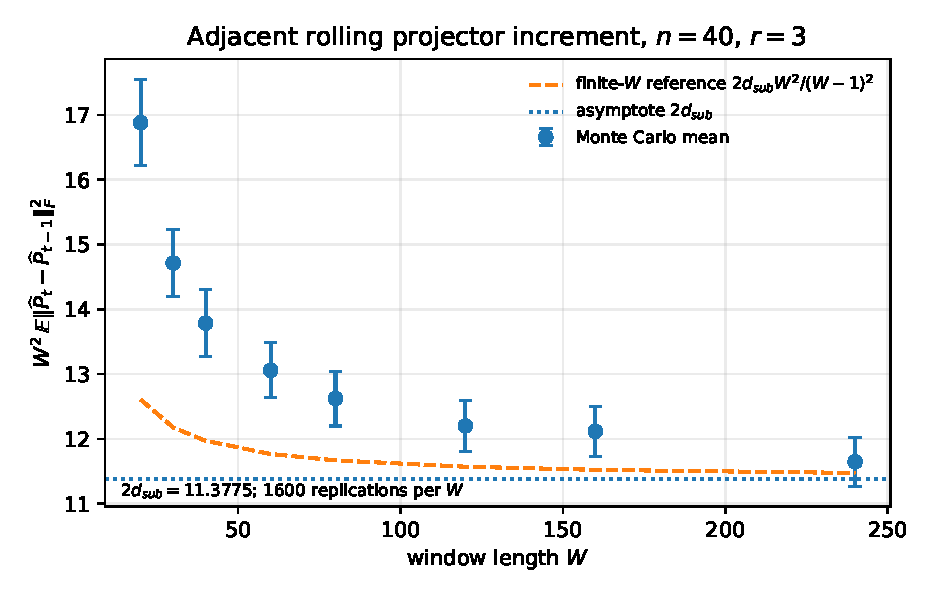
\includegraphics[width=.72\textwidth]{overlap_drift_constant_check.pdf}%
}{%
\fbox{\parbox{.72\textwidth}{\centering Missing file
\texttt{overlap\_drift\_constant\_check.pdf}. Include the Monte Carlo figure
in the source bundle to render this panel.}}%
}
\caption{Monte Carlo check of the leading constant in
Theorem~\ref{thm:adjacentconstantproved}. Error bars are approximate 95\%
Monte Carlo intervals for the scaled mean; the finite-$W$ reference includes
the $\alpha_W^{-2}$ correction, while the horizontal asymptote is
$2\dsub(\Sigma,r)$.}
\label{fig:constantcheck}
\end{figure}

\section{Boundary-driven sharpness}

The adjacent-window lower bound requires a precise target. It is not a lower
bound for arbitrary instantaneous drift, and it is not a claim of nontrivial
recovery below the null fluctuation floor. Under a known static null the
population instantaneous drift $P_t-P_{t-1}$ is zero and the estimator
$\widehat D\equiv0$ has zero risk. Under a fully nonstatic class, instantaneous
drift may be harder than $r/W^2$ because only one new observation is available
at each endpoint. We therefore state the sharp $r/W^2$ lower bound for the
overlap-driven rolling target
\[
D_t^{\mathrm{roll}}
:=P(\bar\Sigma_t)-P(\bar\Sigma_{t-1}),
\]
where $\bar\Sigma_t$ denotes the population window average. Equivalently, the
same construction applies to local path models in which adjacent rolling drift
is generated by the boundary innovation; it should not be read as a statement
about an unrestricted target $P_t-P_{t-1}$.

\begin{proposition}[Boundary-driven rolling-drift lower bound]\label{prop:rollinglower}
Fix $r$ and suppose $n\ge2r+1$. There is a finite family of product Gaussian
adjacent-window experiments $\{\mathbb P_\Theta:\Theta\in\mathcal V\}$ with the
following explicit form. In experiment $\mathbb P_\Theta$, the $W-1$ shared-core
observations are independent $N(0,\Sigma_0)$ vectors, the entering boundary
observation is $N(0,\Sigma_\Theta)$, and the exiting boundary observation is
$N(0,\Sigma_{-\Theta})$, all mutually independent. The covariances are
\[
\Sigma_0=I_n+nP_0,\qquad
\Sigma_{\pm\Theta}=I_n+nP_{\pm\Theta},
\]
where $P_0$ is the coordinate rank-$r$ projector and $P_{\pm\Theta}$ are the
graph projectors constructed in the proof. The boundary covariances satisfy the
bulk-plus-spikes and eigengap conditions uniformly. The corresponding population
window averages
\[
\bar\Sigma_t(\Theta)
=\Sigma_0+\frac1W(\Sigma_\Theta-\Sigma_0),
\qquad
\bar\Sigma_{t-1}(\Theta)
=\Sigma_0+\frac1W(\Sigma_{-\Theta}-\Sigma_0)
\]
have a uniformly separated top-$r$ spectral cluster; their lower cluster is
bounded by $C(1+n/W)$. In particular, if one additionally imposes $W\gtrsim n$,
then the population window averages also satisfy the full bulk-plus-spikes
condition uniformly. There is a threshold
$W_0=W_0(r,\text{spectral constants})$, not depending on $n$, such that for all
$W\ge W_0$, uniformly over $n\ge 2r+1$,
\[
\inf_{\widehat D}\sup_{\Theta\in\mathcal V}
\E_\Theta\norm{\widehat D-D_t^{\mathrm{roll}}(\Theta)}_F^2
\ge
c\frac r{W^2}.
\]
\end{proposition}

\begin{proof}
Let $P_0$ be the coordinate rank-$r$ projector,
\[
P_0=
\begin{pmatrix}
I_r&0\\
0&0
\end{pmatrix},
\qquad
\Sigma_0=I_n+nP_0.
\]
For a matrix $\Theta\in\mathbb R^{(n-r)\times r}$ with sufficiently small
operator norm, define
\[
U_\Theta=
\begin{pmatrix}
I_r\\
\Theta
\end{pmatrix}
(I_r+\Theta^\top\Theta)^{-1/2},
\qquad
P_\Theta=U_\Theta U_\Theta^\top,
\qquad
\Sigma_\Theta=I_n+nP_\Theta.
\]
Every $\Sigma_\Theta$ in this local family has $r$ eigenvalues equal to $n+1$
and $n-r$ eigenvalues equal to $1$, so the boundary covariances have uniform
spike size, bounded bulk, and eigengap.

We consider the adjacent-window experiment in which the $W-1$ shared-core
observations have covariance $\Sigma_0$, the entering boundary observation has
covariance $\Sigma_\Theta$, and the exiting boundary observation has covariance
$\Sigma_{-\Theta}$. Thus
\[
\bar\Sigma_t(\Theta)
=\Sigma_0+\frac1W(\Sigma_\Theta-\Sigma_0),
\qquad
\bar\Sigma_{t-1}(\Theta)
=\Sigma_0+\frac1W(\Sigma_{-\Theta}-\Sigma_0),
\]
and the target is
\[
D_t^{\mathrm{roll}}(\Theta)
=P(\bar\Sigma_t(\Theta))-P(\bar\Sigma_{t-1}(\Theta)).
\]
The window averages retain a uniform top-$r$ eigengap but need not retain an
$O(1)$ lower cluster unless $W$ is at least of order $n$. Indeed,
\[
\bar\Sigma_t(\Theta)=I_n+n\left(\left(1-\frac1W\right)P_0+\frac1W P_\Theta\right),
\]
and Weyl's inequality gives, uniformly over the local chart,
\[
\lambda_r(\bar\Sigma_t(\Theta))\ge n+1-\frac{2n}{W},
\qquad
\lambda_{r+1}(\bar\Sigma_t(\Theta))\le 1+\frac{2n}{W}.
\]
The same bounds hold for $\bar\Sigma_{t-1}(\Theta)$. Hence, for all sufficiently
large $W$, both averages have a top-$r$ eigengap at least a fixed multiple of
$n$, while their lower cluster is bounded by $C(1+n/W)$; in the subregime
$W\gtrsim n$ this is the original $O(1)$ bulk condition.

We first record the local geometry of this target. Let
\[
K(\Theta)=
\begin{pmatrix}
0&\Theta^\top\\
\Theta&0
\end{pmatrix}.
\]
The graph-projector formula gives, uniformly for
$\norm{\Theta}_{\op},\norm{\Theta'}_{\op}\le\varepsilon$,
\[
P_\Theta-P_0=K(\Theta)+E(\Theta),
\qquad
P_{-\Theta}-P_0=-K(\Theta)+E(-\Theta),
\]
with
\[
\norm{E(\Theta)-E(\Theta')}_F
\le C\varepsilon\norm{\Theta-\Theta'}_F.
\]
Indeed, this follows by direct block computation from
$U_\Theta=(I_r,\Theta)^\top(I_r+\Theta^\top\Theta)^{-1/2}$. Writing
$M=(I_r+\Theta^\top\Theta)^{-1/2}$, one has
\[
P_\Theta
=U_\Theta U_\Theta^\top
=
\begin{pmatrix}
M^2 & M^2\Theta^\top\\[2pt]
\Theta M^2 & \Theta M^2\Theta^\top
\end{pmatrix}
=
\begin{pmatrix}
(I_r+\Theta^\top\Theta)^{-1} & (I_r+\Theta^\top\Theta)^{-1}\Theta^\top\\[2pt]
\Theta(I_r+\Theta^\top\Theta)^{-1} & \Theta(I_r+\Theta^\top\Theta)^{-1}\Theta^\top
\end{pmatrix},
\]
so the blocks of $E(\Theta)=P_\Theta-P_0-K(\Theta)$ are
\[
\begin{aligned}
E(\Theta)_{11}&=(I_r+\Theta^\top\Theta)^{-1}-I_r=-\Theta^\top\Theta+O(\norm{\Theta}^4),\\
E(\Theta)_{22}&=\Theta(I_r+\Theta^\top\Theta)^{-1}\Theta^\top=\Theta\Theta^\top+O(\norm{\Theta}^4),\\
E(\Theta)_{12}&=\bigl[(I_r+\Theta^\top\Theta)^{-1}-I_r\bigr]\Theta^\top
=-\Theta^\top\Theta\Theta^\top+O(\norm{\Theta}^5),
\end{aligned}
\]
and $E(\Theta)_{21}=E(\Theta)_{12}^\top$. Thus the diagonal blocks are quadratic
in $\Theta$ and the off-diagonal blocks are cubic; in either case
$E(\Theta)=O(\norm{\Theta}^2)$ and the map $\Theta\mapsto E(\Theta)$ has
$C\varepsilon$-Lipschitz constant on $\norm{\Theta}_{\op}\le\varepsilon$, which is
all that is used below. (The off-diagonal block is governed by
$(I_r+\Theta^\top\Theta)^{-1}$, not by $(I_r+\Theta^\top\Theta)^{-1/2}$, and its
leading correction to $\Theta^\top$ is cubic rather than quadratic.) Since $r$ is
fixed, the constants in this Lipschitz bound are uniform in $n$ on the local
chart.

We now make the projector Taylor expansion at $\Sigma_0$ quantitative. The
top-$r$ eigengap of $\Sigma_0=I_n+nP_0$ equals $n$, so
Lemma~\ref{lem:projectorexpansion} gives, for symmetric $E,E_1,E_2$,
\[
\norm{\mathcal L_{\Sigma_0}(E)}_F\le C_r\frac{\norm E_{\op}}{n},
\qquad
\norm{D^2P(\Sigma_0+H)[E_1,E_2]}_F\le C_r\frac{\norm{E_1}_{\op}\norm{E_2}_{\op}}{n^2},
\]
the second bound holding uniformly for $\norm H_{\op}\le n/4$. Since
$\Sigma_\Theta-\Sigma_{\Theta'}=n(P_\Theta-P_{\Theta'})
=nK(\Theta-\Theta')+n\bigl(E(\Theta)-E(\Theta')\bigr)$, the block expansion of $E$
above yields
\[
\norm{\Sigma_\Theta-\Sigma_{\Theta'}-nK(\Theta-\Theta')}_{\op}
\le Cn\varepsilon\norm{\Theta-\Theta'}_F,
\qquad
\norm{\Sigma_\Theta-\Sigma_0}_{\op}\le Cn\varepsilon .
\]
Because $K(\Theta)$ is supported on the off-diagonal blocks between $P_0$ and
$P_0^\perp$, the reduced-resolvent derivative across the gap $n$ acts by
$\mathcal L_{\Sigma_0}(nK(\Theta)/W)=K(\Theta)/W$. Applying the first-order
expansion to $\bar\Sigma_t(\Theta)=\Sigma_0+W^{-1}(\Sigma_\Theta-\Sigma_0)$, whose
perturbation has operator norm $O(n\varepsilon/W)\le n/4$ for $\varepsilon$ small
and $W\ge W_0$, and controlling the second-order remainder by the displayed
$D^2P$ bound together with the $C\varepsilon$-Lipschitz property of $E$, shows
that the Taylor remainder for this projector is Lipschitz of size $C\varepsilon/W$
in the chart. Therefore
\[
P(\bar\Sigma_t(\Theta))
=P_0+\frac1W K(\Theta)+R_+(\Theta),
\qquad
P(\bar\Sigma_{t-1}(\Theta))
=P_0-\frac1W K(\Theta)+R_-(\Theta),
\]
where, uniformly for $\norm{\Theta}_{\op},\norm{\Theta'}_{\op}\le\varepsilon$,
\[
\norm{R_\pm(\Theta)-R_\pm(\Theta')}_F
\le
\frac{C\varepsilon}{W}\norm{\Theta-\Theta'}_F .
\]
Consequently
\[
D_t^{\mathrm{roll}}(\Theta)-D_t^{\mathrm{roll}}(\Theta')
=\frac{2}{W}K(\Theta-\Theta')+
\bigl(R_+(\Theta)-R_+(\Theta')\bigr)
-
\bigl(R_-(\Theta)-R_-(\Theta')\bigr).
\]
Because $\norm{K(A)}_F=\sqrt2\norm A_F$, choosing $\varepsilon>0$ sufficiently
small gives the bi-Lipschitz lower bound
\begin{equation}\label{eq:local-bilip-lower}
\norm{
D_t^{\mathrm{roll}}(\Theta)-D_t^{\mathrm{roll}}(\Theta')
}_F^2
\ge
\frac c{W^2}\norm{\Theta-\Theta'}_F^2 .
\end{equation}

Now construct the finite subclass promised in the statement. Let $d=r(n-r)$ and
identify $v\in\{-1,1\}^d$ with a matrix
$\Theta_v\in\mathbb R^{(n-r)\times r}$ whose entries are $\pm h$. Set
$\mathcal V=\{\Theta_v:v\in\{-1,1\}^d\}$. Choose
\[
h^2=\frac{\kappa}{n},
\]
where $\kappa>0$ is a sufficiently small constant depending only on $r$ and the
fixed spectral constants. Since $r$ is fixed,
\[
\norm{\Theta_v}_{\op}
\le
\norm{\Theta_v}_F
=h\sqrt{r(n-r)}
\le
C_r\sqrt\kappa,
\]
so the whole hypercube lies in the local neighborhood above when $\kappa$ is
small enough. By \eqref{eq:local-bilip-lower}, for any two vertices,
\begin{equation}\label{eq:hamming-separation}
\norm{
D_t^{\mathrm{roll}}(\Theta_v)-D_t^{\mathrm{roll}}(\Theta_{v'})
}_F^2
\ge
\frac c{W^2}
\norm{\Theta_v-\Theta_{v'}}_F^2
=\frac{4c h^2}{W^2}d_H(v,v'),
\end{equation}
where $d_H$ denotes Hamming distance.

It remains to bound the testing affinity between neighboring vertices. The
$W-1$ shared-core observations have the same law for every $v$ and therefore do
not contribute to the Kullback--Leibler divergence. Only the two boundary
observations depend on $v$.

For two rank-$r$ projectors $P,Q$, set
\[
\Sigma_P=I_n+nP,
\qquad
\Sigma_Q=I_n+nQ.
\]
Since
\[
\Sigma_Q^{-1}=I_n-\frac n{n+1}Q
\]
and $\det(\Sigma_P)=\det(\Sigma_Q)=(n+1)^r$, the Gaussian covariance KL
divergence satisfies
\[
\begin{aligned}
\KL\bigl(N(0,\Sigma_P),N(0,\Sigma_Q)\bigr)
&=
\frac12\left[
\tr(\Sigma_Q^{-1}\Sigma_P)-n
\right]  \\
&=
\frac{n^2}{4(n+1)}\norm{P-Q}_F^2
\le
C n \norm{P-Q}_F^2 .
\end{aligned}
\]
In the local chart,
\[
\norm{P_\Theta-P_{\Theta'}}_F
\le
C\norm{\Theta-\Theta'}_F.
\]
Thus, the entering boundary contribution satisfies, if $v$ and $v'$ differ in
one coordinate,
\[
\KL_{\mathrm{enter}}(\mathbb P_v,\mathbb P_{v'})
\le
C n \norm{\Theta_v-\Theta_{v'}}_F^2
=C n(4h^2)
=C\kappa .
\]
The same bound applies to the exiting boundary covariance
$\Sigma_{-\Theta_v}$ versus $\Sigma_{-\Theta_{v'}}$, and the shared-core part
contributes zero. Hence the full adjacent-window experiment satisfies
\[
\KL(\mathbb P_v,\mathbb P_{v'})
\le 2C\kappa
\le C'\kappa .
\]
Choosing $\kappa$ small enough, Pinsker's inequality
\cite[Ch.~2]{Tsybakov2009} gives a uniform edge affinity bounded away from
zero.

Assouad's lemma \cite{Assouad1983,Yu1997} applied to the hypercube
$\{\Theta_v:v\in\{-1,1\}^d\}$ and the separation
\eqref{eq:hamming-separation} yields
\[
\inf_{\widehat D}
\sup_{v\in\{-1,1\}^d}
\E_v\norm{\widehat D-D_t^{\mathrm{roll}}(\Theta_v)}_F^2
\ge
c\,d\,\frac{h^2}{W^2}.
\]
Since $d=r(n-r)$ and $h^2=\kappa/n$,
\[
d h^2
=r(n-r)\frac{\kappa}{n}
\asymp r
\]
for $n\ge2r+1$. Therefore
\[
\inf_{\widehat D}\sup_{v\in\{-1,1\}^d}
\E_v\norm{\widehat D-D_t^{\mathrm{roll}}(\Theta_v)}_F^2
\ge
c\frac r{W^2}.
\]
This proves the lower bound, with $\mathcal V=\{\Theta_v:v\in\{-1,1\}^d\}$.
\end{proof}

\begin{remark}[Matching upper bound and the limited sharpness claim]\label{rem:matchingupper}
The lower bound of Proposition~\ref{prop:rollinglower} is rate-sharp over the
same local boundary family, but the matching upper bound is intentionally
trivial. The estimator $\widehat D\equiv0$ attains worst-case risk of order
$r/W^2$ because the constructed rolling drift is itself only at the null scale.
Indeed, the first-order projector expansion at $\Sigma_0$ used in the proof
gives, uniformly over the local neighborhood,
\[
\norm{D_t^{\mathrm{roll}}(\Theta)}_F
=\frac1W\norm{2K(\Theta)+W\bigl(R_+(\Theta)-R_-(\Theta)\bigr)}_F
\le
\frac{C}{W}\norm{\Theta}_F,
\]
so that on the hypercube
\[
\sup_{v\in\{-1,1\}^d}\norm{D_t^{\mathrm{roll}}(\Theta_v)}_F^2
\le
\frac{C}{W^2}\norm{\Theta_v}_F^2
=\frac{C}{W^2}\,d h^2
\asymp\frac r{W^2}.
\]
Consequently
\[
\inf_{\widehat D}\sup_{v\in\{-1,1\}^d}
\E_v\norm{\widehat D-D_t^{\mathrm{roll}}(\Theta_v)}_F^2
\le
\sup_{v\in\{-1,1\}^d}\norm{D_t^{\mathrm{roll}}(\Theta_v)}_F^2
\le
C\frac r{W^2},
\]
and Proposition~\ref{prop:rollinglower} gives the reverse inequality up to
constants. Thus the minimax risk over this least-favorable family is exactly of
order $r/W^2$. This should not be read as a nontrivial estimation theorem below
the benchmark of Theorem~\ref{thm:overlapbenchmark}; it says that, when the
rolling signal is manufactured at the same scale as the static-null
fluctuation floor, no estimator can improve the rate, and outputting zero is
already rate-optimal on this least-favorable family.
\end{remark}

\begin{remark}[Instantaneous versus rolling drift]\label{rem:instantaneousvsrolling}
Proposition~\ref{prop:rollinglower} concerns $D_t^{\mathrm{roll}}$, not the
arbitrary instantaneous target $P_t-P_{t-1}$. A lower bound for instantaneous
drift requires an additional local path model linking $P_t-P_{t-1}$ to the
boundary difference seen by the two adjacent rolling windows. Without such a
link the problem can be either easier, as under a known static null, or harder,
as in unrestricted nonstationary models. Thus the sharpness claim in
Proposition~\ref{prop:rollinglower} is intentionally a rolling-target claim.
\end{remark}

\section{Discussion}

The central mechanism in this analysis is the shared-core decomposition of
adjacent rolling windows. It yields a null increment scale that is smaller by
one factor of $W$ than the single-window projector error: the single-window
perturbation uses $W$ noisy observations, whereas the adjacent difference uses
only the entering and exiting observations after the common core cancels. Under
the bulk-plus-spikes scaling this produces the two scales
\[
\text{single-window projector scale } r/W,
\qquad
\text{adjacent overlap drift scale } r/W^2.
\]
We stress that, under the static null, the constant $2\mathfrak d_{\mathrm{sub}}/W^2$
is a \emph{null-fluctuation floor} rather than a measure of any real movement of
the population subspace, which is fixed: it quantifies the noise that genuine
drift must exceed to be detectable.

The lower-bound construction in Proposition~\ref{prop:rollinglower} is separate
from this null calculation: it concerns the rolling target
$D_t^{\mathrm{roll}}$ in a boundary-varying family, and its matching upper
bound is the zero estimator because the constructed signal is already at the
null scale. The construction keeps the boundary covariances in the stated
bulk-plus-spikes class. The population window averages retain a uniformly
separated top-$r$ cluster, which is what the rolling target needs, but their
lower cluster is $O(1+n/W)$; hence the averages themselves satisfy the full
$O(1)$-bulk version of Assumption~\ref{ass:bulkspike} only in the additional
regime $W\gtrsim n$.

The leading constant is not obtained by applying Davis--Kahan
\cite{DavisKahan1970} to two independent windows. It requires conditioning on
the shared core, expanding each endpoint around that same random core, and then
replacing the random-core variance functional by its population limit. Two
distinct calibrations follow from the same conditioning: the magnitude
benchmark $2\mathfrak d_{\mathrm{sub}}/(W-1)^2$ of
Theorem~\ref{thm:adjacentconstantproved}, with limiting shorthand
$2\mathfrak d_{\mathrm{sub}}/W^2$, which is asymptotic and carries the
factor-of-two convention of Remark~\ref{rem:convention}, and the exact
finite-sample sign symmetry of Theorem~\ref{thm:exactrandomization}, which
needs no constant at all and so remains calibrated for a fixed oriented
contrast even when the magnitude scale is in doubt. Sequential use over many
overlapping times, however, still requires the additional dependence handling
described in Remark~\ref{rem:sequentialsign}.

\begin{remark}[Scope: spectral regime and Gaussianity]\label{rem:scope}
Three boundaries of the present analysis are worth stating explicitly.

First, Assumption~\ref{ass:bulkspike} fixes the benign, strongly spiked
regime: $r$ spikes of order $n$ separated from an $O(1)$ bulk by a gap of order
$n$. It
is precisely this $\Theta(n)$ separation that makes the rates dimension-free,
the linearization remainder negligible, and the spectral-difficulty functional
$\mathfrak d_{\mathrm{sub}}=\Theta(r)$. The harder high-dimensional regimes ---
bounded spikes, a shrinking eigengap, or proportional growth with $n/W$ of
constant order, where Baik--Ben Arous--P\'ech\'e phase-transition phenomena and
nontrivial eigenvector inconsistency arise --- are deliberately excluded, and
the constant $2\mathfrak d_{\mathrm{sub}}/W^2$ should not be expected to persist
in that setting.

Second, the conditioning argument requires an exchangeable boundary pair
independent of the shared core. The i.i.d. Gaussian null supplies this directly;
serial dependence, volatility clustering, or deterministic local trends can
make $r_t$ and $r_{t-W}$ nonexchangeable after conditioning on the core, in
which case the exact sign-randomization statement does not apply without an
additional blocking or model-based resampling step.

Third, the \emph{exact constant} is Gaussian. The exact sign-randomization
statement uses only conditional exchangeability of the boundary pair. The
magnitude rate $r/W^2$ is expected to extend beyond Gaussian innovations under
additional assumptions ensuring shared-core eigengap concentration and suitable
quadratic-chaos moment or tail bounds, but that extension is not proved here. At
the purely linearized second-moment level, non-Gaussian innovations would
introduce fourth-cumulant terms; finite fourth moments alone do not give the
full high-dimensional theorem proved here. Thus the constant
$2\mathfrak d_{\mathrm{sub}}$ is specific to the Gaussian Isserlis calculation,
while non-Gaussian boundary innovations generally lead to model-dependent
leading constants.
\end{remark}

\begin{thebibliography}{99}

\bibitem{Assouad1983}
P.~Assouad.
\newblock Deux remarques sur l'estimation.
\newblock {\em C. R. Acad. Sci. Paris S\'er. I Math.}, 296(23):1021--1024, 1983.

\bibitem{AueEtAl2009}
A.~Aue, S.~H\"ormann, L.~Horv\'ath, and M.~Reimherr.
\newblock Break detection in the covariance structure of multivariate time
series models.
\newblock {\em Ann. Statist.}, 37(6B):4046--4087, 2009.

\bibitem{BenaychNadakuditi2011}
F.~Benaych-Georges and R.~R. Nadakuditi.
\newblock The eigenvalues and eigenvectors of finite, low rank perturbations of
large random matrices.
\newblock {\em Adv. Math.}, 227(1):494--521, 2011.

\bibitem{Bhatia1997}
R.~Bhatia.
\newblock {\em Matrix Analysis}, volume 169 of {\em Graduate Texts in
Mathematics}.
\newblock Springer, New York, 1997.

\bibitem{CaiMaWu2013}
T.~T. Cai, Z.~Ma, and Y.~Wu.
\newblock Sparse {PCA}: optimal rates and adaptive estimation.
\newblock {\em Ann. Statist.}, 41(6):3074--3110, 2013.

\bibitem{CaiZhang2018}
T.~T. Cai and A.~Zhang.
\newblock Rate-optimal perturbation bounds for singular subspaces with
applications to high-dimensional statistics.
\newblock {\em Ann. Statist.}, 46(1):60--89, 2018.

\bibitem{DavisKahan1970}
C.~Davis and W.~M. Kahan.
\newblock The rotation of eigenvectors by a perturbation. {III}.
\newblock {\em SIAM J. Numer. Anal.}, 7(1):1--46, 1970.

\bibitem{HsuKakadeZhang2012}
D.~Hsu, S.~M. Kakade, and T.~Zhang.
\newblock A tail inequality for quadratic forms of subgaussian random vectors.
\newblock {\em Electron. Commun. Probab.}, 17(52):1--6, 2012.

\bibitem{Isserlis1918}
L.~Isserlis.
\newblock On a formula for the product-moment coefficient of any order of a
normal frequency distribution in any number of variables.
\newblock {\em Biometrika}, 12(1/2):134--139, 1918.

\bibitem{Janson1997}
S.~Janson.
\newblock {\em Gaussian Hilbert Spaces}, volume 129 of {\em Cambridge Tracts in
Mathematics}.
\newblock Cambridge University Press, Cambridge, 1997.

\bibitem{Johnstone2001}
I.~M. Johnstone.
\newblock On the distribution of the largest eigenvalue in principal components
analysis.
\newblock {\em Ann. Statist.}, 29(2):295--327, 2001.

\bibitem{Kato1995}
T.~Kato.
\newblock {\em Perturbation Theory for Linear Operators}.
\newblock Classics in Mathematics. Springer, Berlin, reprint of the 1980
edition, 1995.

\bibitem{KoltchinskiiLounici2017}
V.~Koltchinskii and K.~Lounici.
\newblock Concentration inequalities and moment bounds for sample covariance
operators.
\newblock {\em Bernoulli}, 23(1):110--133, 2017.

\bibitem{LaurentMassart2000}
B.~Laurent and P.~Massart.
\newblock Adaptive estimation of a quadratic functional by model selection.
\newblock {\em Ann. Statist.}, 28(5):1302--1338, 2000.

\bibitem{LehmannRomano2005}
E.~L. Lehmann and J.~P. Romano.
\newblock {\em Testing Statistical Hypotheses}.
\newblock Springer Texts in Statistics. Springer, New York, third edition,
2005.

\bibitem{Nelson1973}
E.~Nelson.
\newblock The free {M}arkoff field.
\newblock {\em J. Funct. Anal.}, 12(2):211--227, 1973.

\bibitem{Paul2007}
D.~Paul.
\newblock Asymptotics of sample eigenstructure for a large dimensional spiked
covariance model.
\newblock {\em Statist. Sinica}, 17(4):1617--1642, 2007.

\bibitem{StewartSun1990}
G.~W. Stewart and J.-G. Sun.
\newblock {\em Matrix Perturbation Theory}.
\newblock Academic Press, Boston, 1990.

\bibitem{Tsybakov2009}
A.~B. Tsybakov.
\newblock {\em Introduction to Nonparametric Estimation}.
\newblock Springer Series in Statistics. Springer, New York, 2009.

\bibitem{Vershynin2018}
R.~Vershynin.
\newblock {\em High-Dimensional Probability: An Introduction with Applications
in Data Science}, volume 47 of {\em Cambridge Series in Statistical and
Probabilistic Mathematics}.
\newblock Cambridge University Press, Cambridge, 2018.

\bibitem{VuLei2013}
V.~Q. Vu and J.~Lei.
\newblock Minimax sparse principal subspace estimation in high dimensions.
\newblock {\em Ann. Statist.}, 41(6):2905--2947, 2013.

\bibitem{WangYuRinaldo2021}
D.~Wang, Y.~Yu, and A.~Rinaldo.
\newblock Optimal covariance change point localization in high dimensions.
\newblock {\em Bernoulli}, 27(1):554--575, 2021.

\bibitem{Wedin1972}
P.-{\AA}. Wedin.
\newblock Perturbation bounds in connection with singular value decomposition.
\newblock {\em BIT}, 12(1):99--111, 1972.

\bibitem{Yu1997}
B.~Yu.
\newblock Assouad, {F}ano, and {L}e {C}am.
\newblock In {\em Festschrift for Lucien Le Cam}, pages 423--435. Springer, New
York, 1997.

\end{thebibliography}

\end{document}
